% $Id: patches.tex 5960 2018-03-13 00:18:07Z mskala $

%
% MSK 011 patch ideas
% Copyright (C) 2018  Matthew Skala
%
% This program is free software: you can redistribute it and/or modify
% it under the terms of the GNU General Public License as published by
% the Free Software Foundation, version 3.
%
% This program is distributed in the hope that it will be useful,
% but WITHOUT ANY WARRANTY; without even the implied warranty of
% MERCHANTABILITY or FITNESS FOR A PARTICULAR PURPOSE.  See the
% GNU General Public License for more details.
%
% You should have received a copy of the GNU General Public License
% along with this program.  If not, see <http://www.gnu.org/licenses/>.
%
% Matthew Skala
% https://northcoastsynthesis.com/
% mskala@northcoastsynthesis.com
%

\chapter{Patch ideas}

The basic operation of the MSK~011 is very simple:  it mixes signals.  Here,
an oscillator and noise source are combined before being fed into a filter. 
Using the AC-coupled output is appropriate for audio signals where no DC
offset is desirable.  Remember to turn down the top and bottom knobs, which
function as offset generators, if they are not in use.

\nopagebreak\noindent
{\hspace*{\fill}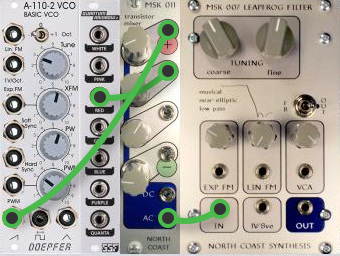
\includegraphics[scale=0.6]{patch1.png}\hspace*{\fill}\par} 

This patch combines three slow sine waves from an MSK~010 to generate a
melody.  The top knob is left unpatched and can be turned up to generate a
positive offset, shifting these bipolar signals into the 0$\ldots$5V range
needed by the quantizer.  Note use of the DC-coupled output to preserve the
voltage levels.

\nopagebreak\noindent
{\hspace*{\fill}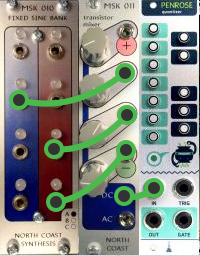
\includegraphics[scale=0.6]{patch2.png}\hspace*{\fill}\par} 

Applying a DC offset (top and bottom knobs), then removing it with the
AC-coupled output, allows the module to clip signals in a controlled way on
one side, for even-harmonic distortion.

\nopagebreak\noindent
{\hspace*{\fill}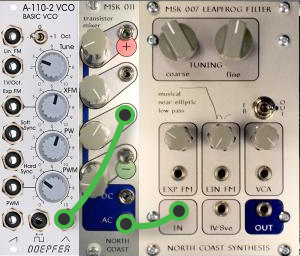
\includegraphics[scale=0.6]{patch3.png}\hspace*{\fill}\par} 

Each channel has maximum gain somewhat over unity, but to boost a signal
further, you can feed it into two or more channels and turn them all up. 
Shown here with a passive cable-adapter module; you might use a patch like
this to boost an external signal a little bit.

\nopagebreak\noindent
{\hspace*{\fill}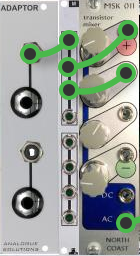
\includegraphics[scale=0.6]{patch4.png}\hspace*{\fill}\par} 

For more gain, use feedback from the DC-coupled output to a channel and
then take the result from the AC-coupled output.  This arrangement will
amplify any DC offset too, so it may require some careful adjustment of the
top or bottom knobs to cancel out that effect.  Voltage gains of up to 10
seem to be reasonably stable; in principle there is no limit.  Feedback
through the AC-coupled output would cancel most of the offset, but may have
phase problems.  The mixer will probably not oscillate under any purely
self-patched configuration, though (like any mixer) it could be combined
with other modules, such as filters, into more complicated feedback patches.

\nopagebreak\noindent
{\hspace*{\fill}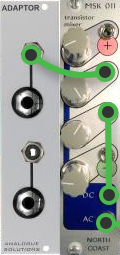
\includegraphics[scale=0.6]{patch5.png}\hspace*{\fill}\par} 
